\documentclass[tikz]{standalone}
\usepackage{amsmath,amssymb}
\usepackage{graphicx} % Required for inserting images
\usepackage{booktabs}
\usepackage{tabularx}
\usepackage{circuitikz}

\usetikzlibrary{positioning}
\usetikzlibrary{shapes,arrows} 
\tikzstyle{block} = [draw, fill=blue!20, rectangle, minimum height=3em, minimum width=4em]
\tikzstyle{controller} = [draw, fill=green!20, rectangle, minimum height=3em, minimum width=4em]
\tikzstyle{sum} = [draw, fill=blue!20, circle, node distance=1cm]
\tikzstyle{input} = [coordinate]
\tikzstyle{output} = [coordinate]
\begin{document}
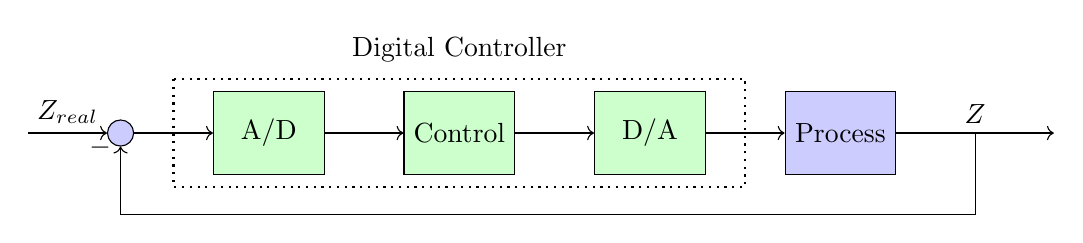
\begin{tikzpicture}[auto]
% Nodes
\node [input] (input) {};
\node [sum, right = 1cm of input] (sum) {};
\node [controller, right = 1cm of sum] (con1) {A/D};
\node [controller, right = 1cm of con1] (con2) {Control};
\node [controller, right = 1cm of con2] (system2) {D/A};
\node [block, right = 1cm of system2] (system3) {Process};
\node [output, right = 2cm of system3] (output) {};
\node [input, below = 0.5cm of con2] (m) {};
% Arrows
\draw [draw,->] (input) -- node {$Z_{real}$} (sum);
\draw [->] (sum) -- (con1);
\draw [->] (con1) -- (con2);
\draw [->] (con2) -- node {$$} (system2);
\draw [->] (system2) -- node {$$} (system3);
\draw [->] (system3) -- node (y) {$Z$}(output);
\draw [-] (y) |- (m) {} ;
\draw [->] (m) -| node[pos=0.99] {$-$}  node [near end] {} (sum);
\draw[thick,dotted]     ($(con1.north west)+(-0.5,0.15)$) rectangle ($(system2.south east)+(0.5,-0.15)$);
\node [above = 0.25cm of con2] {Digital Controller};
%\node [above = of near end] {+};
\end{tikzpicture}
\end{document}